\documentclass[11pt]{article}
\usepackage{ucs}
\usepackage[utf8x]{inputenc}
\usepackage{changepage}
\usepackage{graphicx}
\usepackage{amsmath}
\usepackage{gensymb}
\usepackage{amssymb}
\usepackage{enumerate}
\usepackage{tabularx}
\usepackage{lipsum}

\oddsidemargin 0.0in
\evensidemargin 0.0in
\textwidth 6.27in
\headheight 1.0in
\topmargin 0.0in
\headheight 0.0in
\headsep 0.0in
%\textheight 9.69in
\textheight 9.00in

\setlength\parindent{0pt}

\newenvironment{myenv}{\begin{adjustwidth}{0.4in}{0.4in}}{\end{adjustwidth}}
\renewcommand{\abstractname}{Anotācija}
\renewcommand\refname{Atsauces}

\newenvironment{uzdevums}[1][\unskip]{%
\vspace{3mm}
\noindent
\textbf{#1:}
\noindent}
{}

\newcommand{\subf}[2]{%
  {\small\begin{tabular}[t]{@{}c@{}}
  #1\\#2
  \end{tabular}}%
}



\newcounter{alphnum}
\newenvironment{alphlist}{\begin{list}{(\Alph{alphnum})}{\usecounter{alphnum}\setlength{\leftmargin}{2.5em}} \rm}{\end{list}}


\makeatletter
\let\saved@bibitem\@bibitem
\makeatother

\usepackage{bibentry}
%\usepackage{hyperref}


\begin{document}

\begin{center}
{\Large \bf Jautājumi NT008 (mazākais kopīgais dalāmais u.c.)}
\end{center}

\begin{uzdevums}[AOPS.INT.5.1]
Cik ir pozitīvu skaitļu, kas nepārsniedz 100, kas ir daudzkārtņi skaitlim $2$ vai $3$, bet ne skaitlim $4$. 
\end{uzdevums}




\begin{tabular}{@{}ll@{}} 
\begin{minipage}{0.7\columnwidth}
\begin{uzdevums}[AOPS.INT.5.2a]
(Ieslēgšanas-izslēgšanas princips). Cik ir skaitļu no $1$ līdz $60$, kuri\\
(a) dalās ar vismaz vienu no skaitļiem $2$ vai $3$? \\
(b) dalās ar $2$ vai $3$, bet ne ar abiem diviem.\\
(c) dalās ar $2$, bet nedalās ar $3$?\\ 
(d) dalās ar $3$, bet nedalās ar $2$?\\
(e) nedalās ne ar $2$, ne ar $3$?
\end{uzdevums}
\end{minipage} &
\begin{minipage}{0.25\columnwidth}
\begin{center}
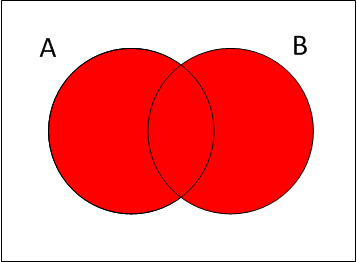
\includegraphics[width=1.5in]{test08-2a.png}
\end{center}
\end{minipage}
\end{tabular}


\begin{tabular}{@{}ll@{}} 
\begin{minipage}{0.7\columnwidth}
\begin{uzdevums}[AOPS.INT.5.3a]
(Ieslēgšanas-izslēgšanas princips). Cik ir skaitļu no $1$ līdz $60$, kuri dalās 
ar vismaz vienu no skaitļiem $2$, $3$ vai $5$? 
Pēterītis izrēķināja, ka ${\displaystyle 60 \cdot \left( 1 - \frac{1}{2} \right)
 \cdot \left( 1 - \frac{1}{3} \right) \cdot \left( 1 - \frac{1}{5} \right) = 16}$. 
Viņš apgalvo, ka tas sakrīt ar to skaitļu skaitu no 
$1$ līdz $60$, kuri nedalās ne ar $2$, ne ar $3$, ne ar $5$. Vai Pēterītim taisnība?
\end{uzdevums}
\end{minipage} &
\begin{minipage}{0.25\columnwidth}
\begin{center}
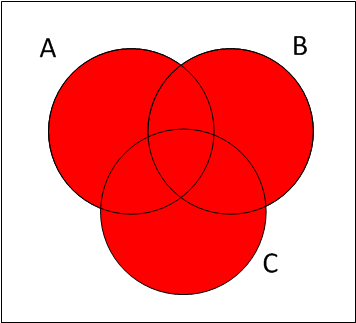
\includegraphics[width=1.5in]{test08-3a.png}
\end{center}
\end{minipage}
\end{tabular}






\begin{uzdevums}[AOPS.INT.5.2]
Planētām $X$, $Y$ un $Z$ vajag attiecīgi $360$, $450$ un $540$ dienas, lai veiktu pilnu apli ap to pašu 
sauli. Ja visas trīs planētas sākumā ir sarindojušās uz tā paša stara (kuram saule ir sākumpunkts), 
kāds ir mazākais pozitīvais dienu skaits, pirms viņas nonāks šajā pašā sākuma stāvoklī? 
\end{uzdevums}


\begin{uzdevums}[AOPS.INT.5.3]
Ar $\gcd(a, b)$ apzīmēsim skaitļu $a$ un $B$ lielāko kopīgo dalītāju, un 
ar $\operatorname{lcm}(c,d)$ apzīmēsim mazāko kopīgo dalāmo skaitļiem $c$ un $d$. 
Cik ir $\gcd(\operatorname{lcm}(8,14),\operatorname{lcm}(7,12))$?
\end{uzdevums}


\begin{uzdevums}[AOPS.INT.5.4]
Ar $A$ apzīmējam visus tos skaitļus, ko var izteikt kā triju pēc kārtas sekojošu naturālu skaitļu summu. 
Kāds ir lielākais kopīgais dalītājs visiem skaitļiem kopā $A$? 
\end{uzdevums}


\begin{uzdevums}[AOPS.INT.5.5]
Kāds ir lielākais kopīgais dalītājs skaitļiem $7979$ un $3713$? (Ieteicams no lielākā skaitļa atņemt kādu mazākā skaitļa 
daudzkārtni, pēc tam - lielāko skaitli aizstāt ar atlikumu, utt.). 
\end{uzdevums}

\begin{uzdevums}[AOPS.INT.5.2.3]
Karlana novieto 600 lodītes $m$ kastēs tā, lai katrā kastē būtu vienāds skaits lodīšu. 
Ir vairāk nekā viena kaste, un katrā kastē ir vairāk nekā viena lodīte. 
Cik dažādām $m$ vērtībām to var izdarīt? 
\end{uzdevums}

\begin{uzdevums}[AOPS.INT.5.4]
Cik daudzi no skaitļa 168 pozitīvajiem dalītājiem ir pāru skaitļi?
\end{uzdevums}

\begin{uzdevums}[AOPS.INT.5.6]
Cik daudzi no skaitļa $5400$ dalītājiem nav daudzkārtņi nevienam pilnam kvadrātam lielākam par $1$? 
\end{uzdevums}

\end{document}